\documentclass[11pt, letterpaper]{article}

% === 页边距：四边均 ≥ 1英寸 ===
\usepackage[letterpaper, top=1in, bottom=1in, left=1in, right=1in]{geometry}

% === 段落间距 ===
\setlength{\parskip}{6pt}
\setlength{\parindent}{0pt}

% === 数学环境与超链接 ===
\usepackage{amsmath}
\usepackage{graphicx}
\usepackage{hyperref}

\begin{document}

% === 标题、作者 ===
\title{When Fairness Metrics Disagree Under Shift: A Stylized Case Study of a Medical Follow-up Risk Score under Hospital Deployment Shift}
\author{Meixuan Chen \\ The Edward S. Rogers Sr. Department of Electrical \& Computer Engineering \\ University of Toronto \\meixan.chen@mail.utoronto.ca}
\maketitle


\section{Introduction}

Group fairness metrics are typically defined under a fixed data-generating process, yet real-world deployments—such as moving a medical follow-up risk score across hospitals—involve distribution shifts that can make these metrics behave unpredictably. In this project, we ask: (1) how do standard group fairness metrics behave under controlled shifts even when the underlying classifier remains fixed? (2) under what conditions can demographic parity remain stable or appear favorable while error-based metrics degrade? and (3) how do importance reweighting, post-hoc threshold adjustment, and target-distribution retraining affect fairness distortion and what trade-offs do they incur? We address these questions via a synthetic simulation framework mimicking a cross-hospital deployment, which allows us to systematically sweep over shift types and magnitudes.

\section{Related Work}
Fairness under non-stationary environments has been studied in several recent works. Asiaee and Aryan (2026) examined invariance under group-conditional prior shifts, while Chen et al. (2022) studied fairness transferability under bounded shifts. Barrainkua et al. (2022) and Shao et al. (2024) provided comprehensive surveys on preserving fairness guarantees and supervised fairness under distribution shifts. However, existing work rarely dissects, under a unified medical deployment simulation, how a static demographic parity value can systematically mask the degradation of error-based metrics—the central gap our study addresses.

\section{Method}

\subsection{Distribution shift mechanisms}
\label{sec:shift_mechanisms}

We consider three families of controlled distribution shift implemented via \texttt{generate\_data}: (i) group-conditioned base-rate shift, (ii) pure group-specific covariate shift, and (iii) group-specific label noise shift. For label-noise experiments, the simulator retains both the clean synthetic outcome $Y^*$ and the recorded outcome $\tilde{Y}$. The source classifier is held fixed for the diagnostic baseline, while mitigation experiments additionally evaluate reweighted training, post-hoc thresholding, and target-distribution retraining. Full mathematical definitions of each shift mechanism are deferred to Appendix \ref{app:a}.

\subsection{Fairness and calibration metrics}
\label{sec:metrics}

We report standard fairness quantities via \texttt{fairlearn.metrics}: demographic parity difference (absolute difference in positive prediction rates), equalized odds difference (worst-case TPR/FPR discrepancy), and the true-positive-rate gap (equal-opportunity violation). We also track global and group-wise expected calibration error (ECE) and the ECE gap to capture calibration disparities. Formal definitions of all metrics are provided in Appendix \ref{app:b}.

\subsection{Mitigation strategies under different target-data access regimes}
\label{sec:mitigations}

Rather than treating the following interventions as interchangeable fixes, we explicitly distinguish them by their target-domain \emph{information requirements} and the shift types for which they are theoretically justified.

\begin{itemize}
    \item \textbf{KDE Importance Reweighting (unsupervised, covariate-shift specific).} 
    This method requires only unlabeled target covariates $X_{\text{target}}$. It estimates the density ratio $w(x)=\hat{p}_{\text{target}}(x)/\hat{p}_{\text{train}}(x)$ via kernel density estimation and reweights the logistic loss accordingly. 
    \emph{Crucially, this intervention is theoretically justified only under pure covariate shift}, where $P(Y|X)$ remains invariant. Under label-noise or prior shifts, $P(Y|X)$ changes, and density-ratio reweighting cannot, in general, correct the resulting fairness distortion. We include it precisely to demonstrate this boundary.

    \item \textbf{Post-hoc Threshold Adjustment (labeled target calibration, equal-opportunity targeting).} 
    This method requires target calibration examples, recorded outcomes $\tilde{Y}$, and group labels $S$. It selects group-specific thresholds to raise the lower TPR toward the higher group's baseline. It does not require retraining the model, but it also does not enforce full equalized odds and can inadvertently increase the FPR gap, as we will show.

    \item \textbf{Target-Distribution Retraining (fully supervised reference).} 
    This method requires a labeled target training set $(X,\tilde{Y})$. It retrains the same logistic model on shifted data and shows what standard target-domain ERM attains when target labels are available. Group labels $S$ are needed to evaluate group fairness, but the present ERM training objective does not use them. Target retraining is not a fairness-specific algorithm or a guaranteed upper bound; it is a supervised reference for the other access regimes.
\end{itemize}

Detailed implementation of each strategy is given in Appendix \ref{app:c}.

\section{Experimental Setup}

\subsection{Shift parameter grid}
\label{sec:setup}

We sweep over the following grids:
\begin{itemize}
    \item Group-conditioned base-rate shift: \(\alpha \in [0, 1]\) with 11 steps.
    \item Covariate shift: \(\gamma \in [1, 4]\) with 10 steps.
    \item Asymmetric label noise: \(\beta \in [0, 0.3]\) with 10 steps.
    \item Joint danger-zone grid: all $11\times10$ combinations of $(\alpha,\beta)$, evaluated over five seeds.
\end{itemize}

Implementation details (sample sizes, classifier hyperparameters, ECE binning, and random seed) are reported in Appendix \ref{app:d}.

\section{Results}

\subsection{Key empirical findings}
\label{sec:results}

Across all three shift families, we observe that demographic parity, error-based metrics, and calibration can move in markedly different directions. Our main results are summarized below. %Baseline phase diagrams, mitigation comparisons, and the target-retraining supplementary figure are saved in \texttt{outputs/figures/}.

\subsubsection{Diagnosis (RQ1 \& RQ2):}
\begin{itemize}
    \item Under \textbf{group-conditioned base-rate shift}, DP increases from 0.01 to 0.26 as \(\alpha\) goes from 0 to 1, while the TPR gap remains between approximately 0.03 and 0.06. The two metric families therefore react very differently to the same prevalence change.

    \item Under \textbf{pure covariate shift}, DP grows from 0.012 to 0.156, while EO and the TPR gap reach 0.233 at \(\gamma=4\). The ECE gap remains below 0.008 because the conditional label mechanism is unchanged and correctly represented by the logistic model. Fairness gaps can therefore grow even when target-domain calibration and balanced accuracy remain strong.

    \item Under \textbf{asymmetric label noise}, DP stays flat at 0.012 even as the TPR gap computed using recorded labels $\tilde{Y}$ grows from 0.032 to 0.176. Because predictions and clean outcomes do not change with $\beta$, this is primarily a measurement distortion: a dashboard using recorded outcomes can report sharply worsening equal opportunity even when the corresponding clean-outcome TPR gap remains stable.
\end{itemize}

\subsubsection{Mitigation (RQ3):}
\begin{itemize}
    \item \textbf{KDE Reweighting:} Under the matched pure covariate shift, the ESS fraction remains between 0.781 and 0.916, but the weighted and frozen curves are nearly identical. This is expected here: $P(Y\mid X,S)$ is invariant and correctly represented by the logistic model, so source and target risk minimizers nearly coincide. Importance weighting remains theoretically appropriate for target-risk correction, but it does not erase group fairness gaps caused by the changed target covariate distribution. Results under prior shift and label noise are retained only as negative controls in the appendix, since the covariate-shift assumption does not hold there.

    \item \textbf{Threshold Adjustment:} Under pure covariate shift it reduces the maximum TPR gap from 0.233 to 0.046, yet the maximum EO difference rises from 0.233 to 0.430 because the FPR gap grows. At $\gamma=4$, balanced accuracy falls from 0.894 for the frozen model to 0.841 after thresholding. Under label noise it lowers the maximum recorded-label TPR gap from 0.176 to 0.030 but raises DP from approximately 0.012 to as much as 0.178.

    \item \textbf{Target Retraining:} Under severe pure covariate shift ($\gamma=4$), target ERM closely matches the frozen model: balanced accuracy is 0.895 versus 0.894, and the TPR gap is 0.221 versus 0.233. This supervised reference confirms that retraining the same correctly specified model offers little additional benefit. Under label noise, retraining keeps DP low but only modestly changes EO.
\end{itemize}

Figure~\ref{fig:access_regimes} compares these methods only under the shift for which KDE weighting is theoretically matched and labels every curve by its target-data requirement.

\begin{figure}[htbp]
    \centering
    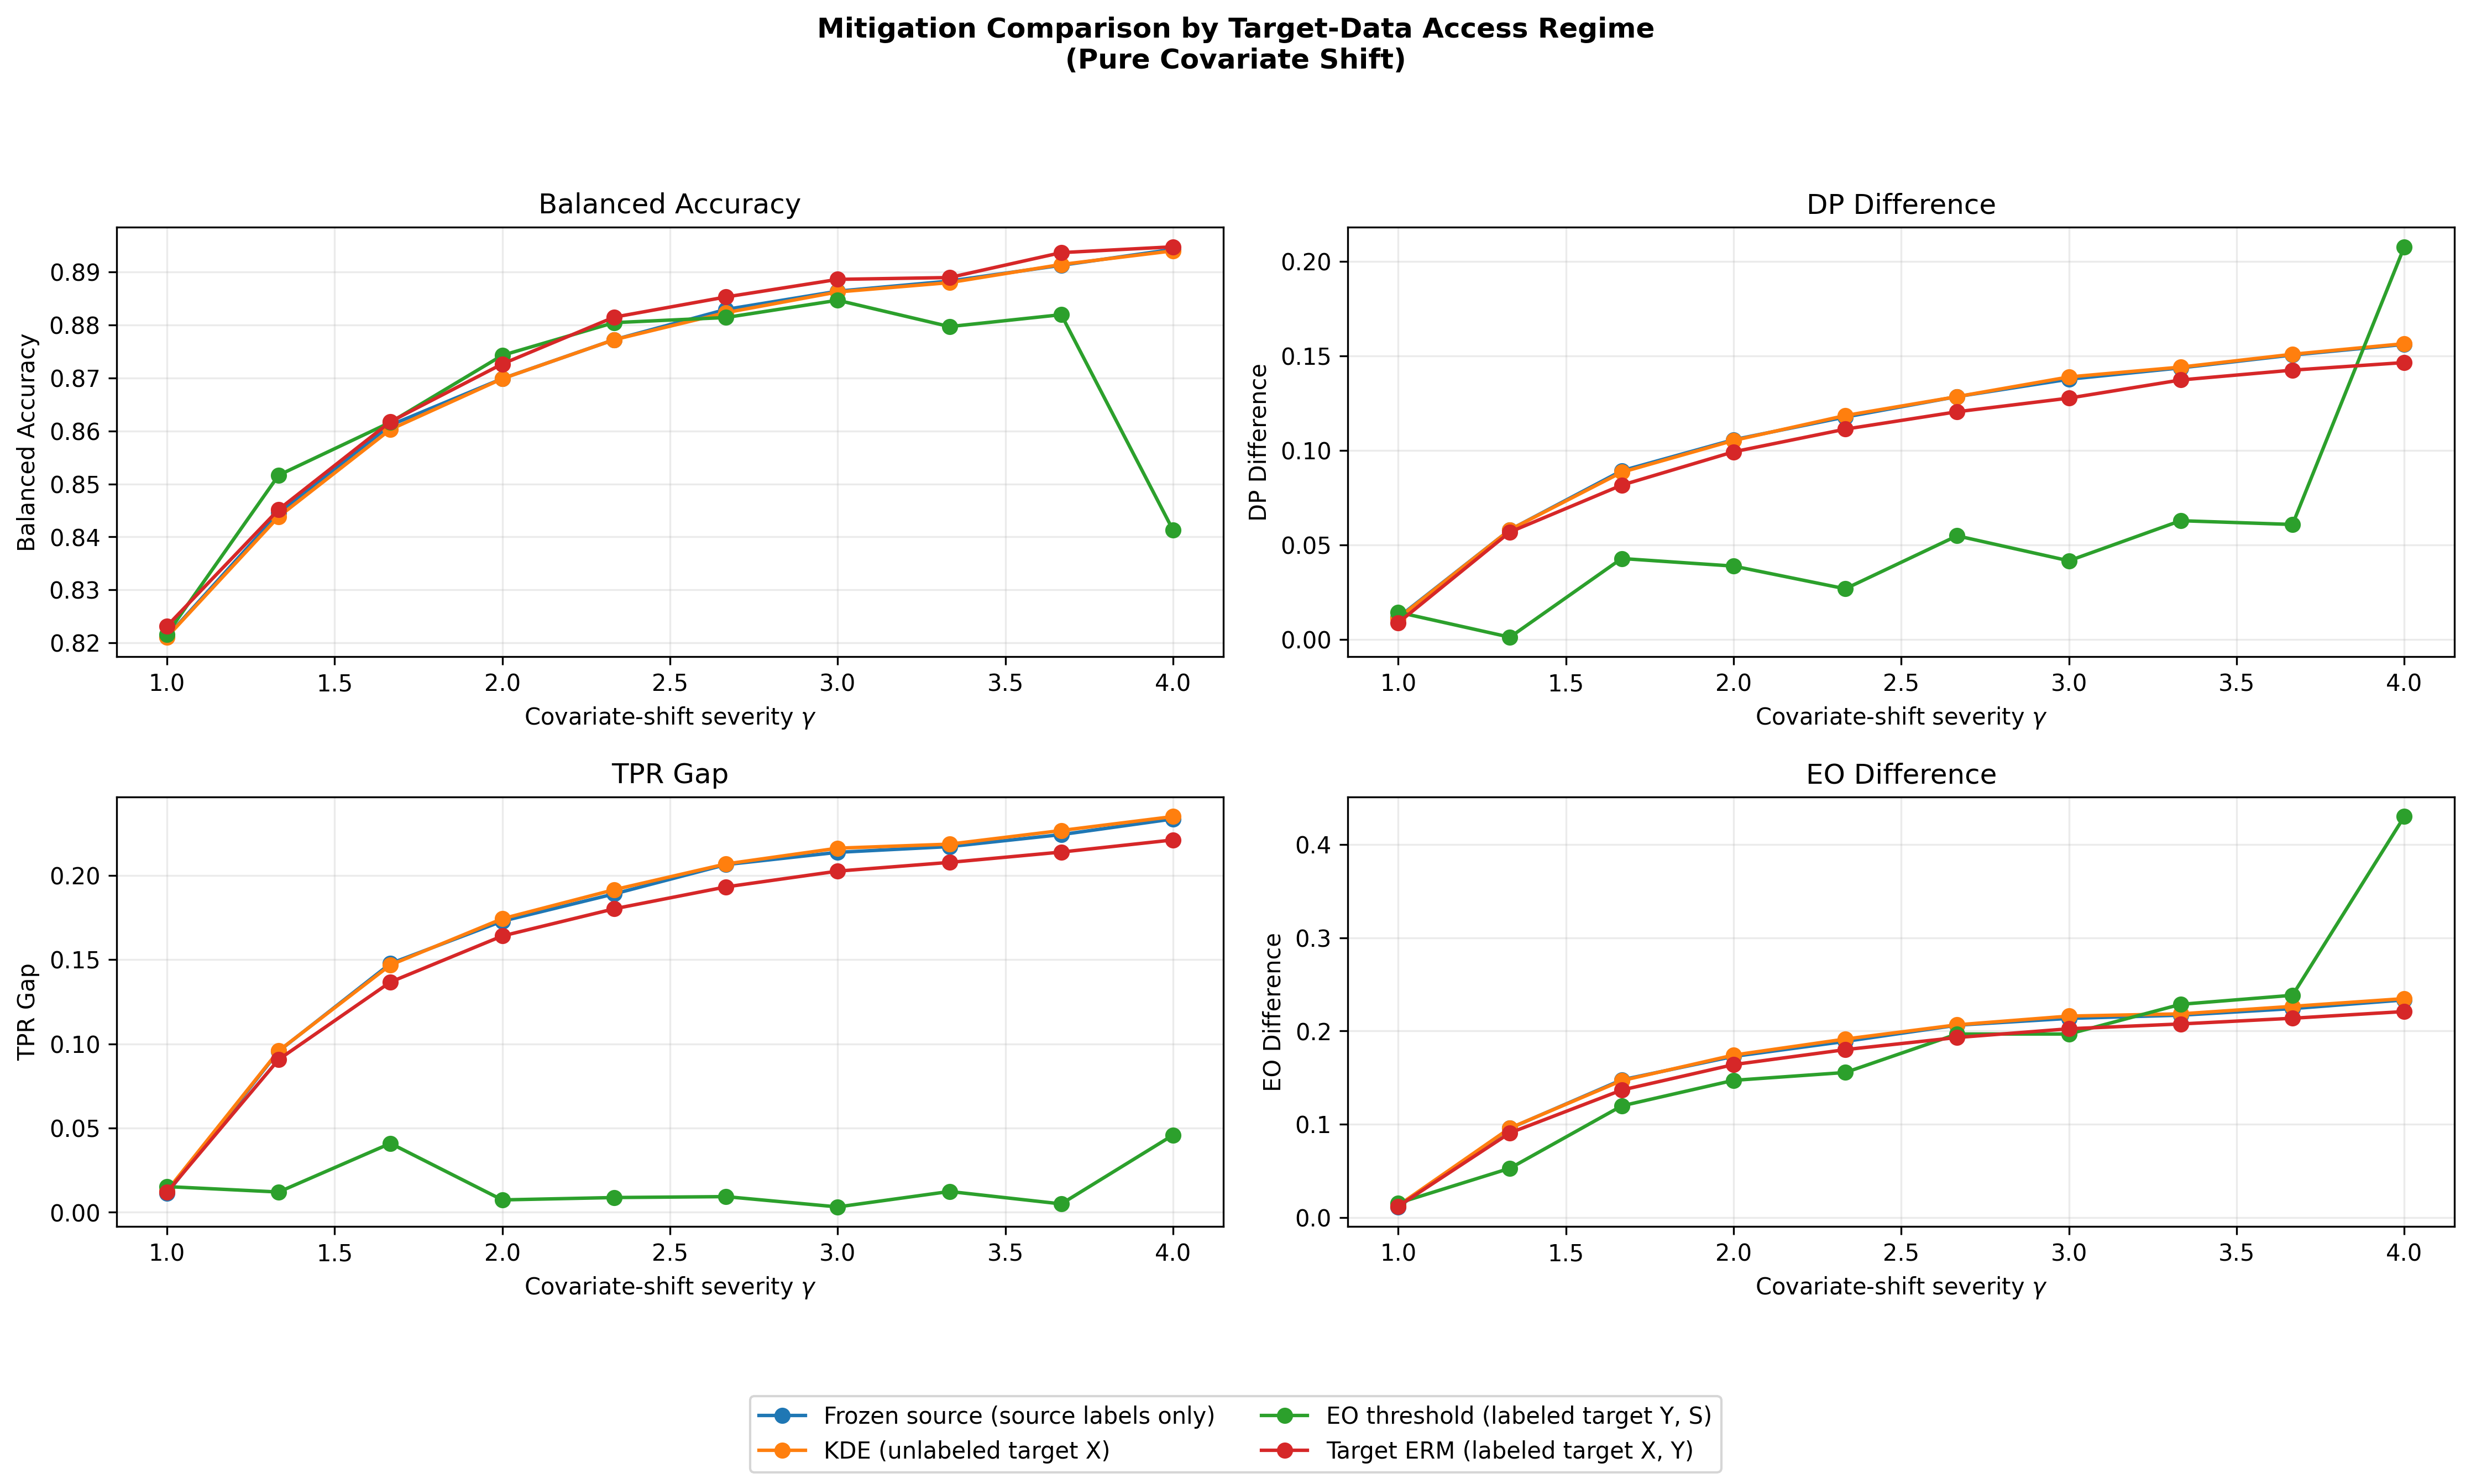
\includegraphics[width=0.98\textwidth]{figures/mitigation_access_regimes_covariate.png}
    \caption{Mitigation comparison under pure covariate shift, organized by target-data access. KDE uses only unlabeled target covariates; equal-opportunity thresholding uses recorded target outcomes and group labels on a calibration set; target ERM uses labeled target training data. The methods are therefore access regimes rather than interchangeable fixes.}
    \label{fig:access_regimes}
\end{figure}

\subsection{Operational definition of the danger zone and phase-diagram analysis}

For each cell of the joint grid, changes are defined relative to the no-shift configuration:
\[
\Delta_D(\alpha,\beta)=\mathrm{DP}(\alpha,\beta)-\mathrm{DP}(0,0),
\]
\[
\Delta_T(\alpha,\beta)=\mathrm{TPRGap}_{\tilde{Y}}(\alpha,\beta)-\mathrm{TPRGap}_{\tilde{Y}}(0,0).
\]
We define an operational \emph{metric-monitoring danger zone} by
\[
\Delta_T\ge 0.05
\quad\land\quad
\left[\Delta_D\le0.02\ \lor\ \Delta_T\ge2\max(\Delta_D,0)\right].
\]
Thus, recorded-label TPR disparity must deteriorate by at least five percentage points while DP either remains stable within two percentage points or changes at less than half the TPR-gap rate. These thresholds are fixed before inspecting individual cells. A cell is reported as dangerous when the condition holds in at least three of five seeds, preventing small sign changes from determining the boundary.

Our main analysis sweeps the joint space of prior shift ($\alpha$) and label-noise severity ($\beta$). Figure~\ref{fig:danger_zone}(a) shows 20 dangerous cells out of 110. They emerge from $\beta\approx0.17$ onward and concentrate at lower $\alpha$, where label noise changes the recorded-label TPR gap while DP remains comparatively insensitive. At larger $\alpha$, DP itself rises substantially, so the discrepancy is no longer hidden from a DP-only monitor.

Because the simulator retains clean outcomes, Figure~\ref{fig:danger_zone}(b) separately compares fairness measured using $\tilde{Y}$ with fairness measured using $Y^*$. In 78 of 110 cells, the recorded and clean TPR gaps differ by at least five percentage points in a majority of seeds. The maximum recorded-label TPR-gap increase is 0.338, whereas the maximum clean-outcome increase is only 0.021. This distinction prevents a recorded-label monitoring failure from being over-interpreted as direct evidence of unequal latent clinical need.

\begin{figure}[htbp]
    \centering
    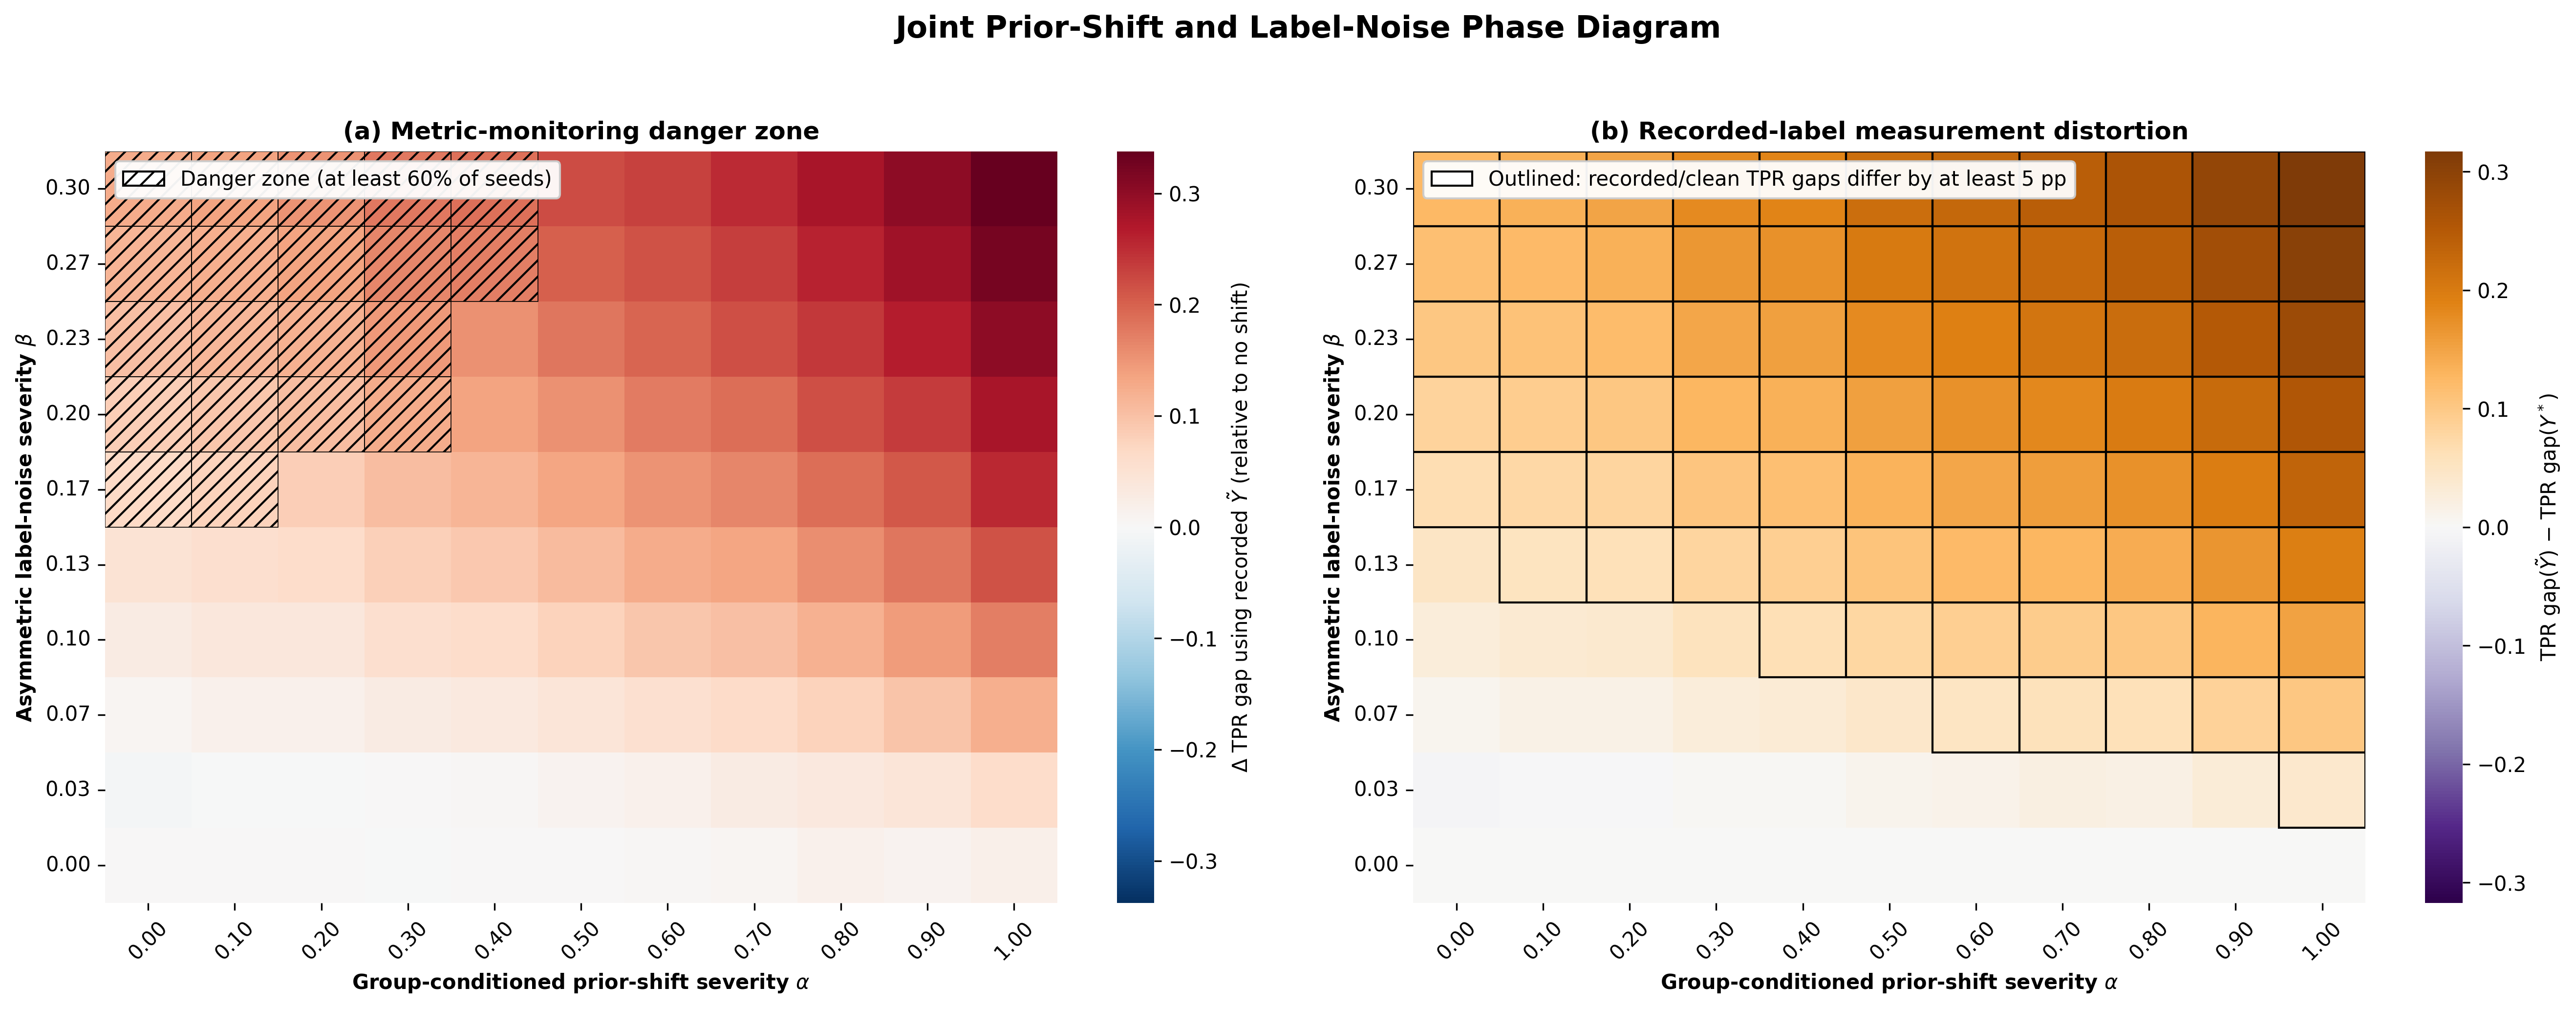
\includegraphics[width=1.0\textwidth]{figures/danger_zone_phase_diagram.png}
    \caption{Joint prior-shift and label-noise phase diagram. Panel (a) colors the change in TPR gap computed using recorded outcomes $\tilde{Y}$ and hatches cells satisfying the pre-specified danger-zone definition in at least three of five seeds. Panel (b) shows the difference between recorded-label and clean-outcome TPR gaps; outlined cells differ by at least five percentage points in at least three seeds.}
    \label{fig:danger_zone}
\end{figure}

We emphasize regions where demographic parity remains stable or changes slowly while error-based metrics such as EO and the TPR gap worsen. The mitigation plots also show the converse: explicitly reducing the TPR gap can increase DP or the FPR-driven EO difference. Thus, a favorable movement in one fairness quantity need not correspond to uniformly fairer behavior.

\section{Conclusion and Future Work}

Our simulations reveal several patterns. A stable or comparatively favorable demographic-parity value can mask large changes in error-based fairness; asymmetric corruption of recorded outcomes is the clearest example. In practice, a hospital dashboard that monitors only demographic parity can miss changes in recorded-label error disparities, while a dashboard that treats recorded outcomes as ground truth can also mistake documentation distortion for a change in latent clinical need. A deployed follow-up score should therefore track DP, TPR gaps, calibration, and data-quality indicators side by side, with each metric tied to the outcome definition used to compute it. Different metrics can disagree not only in level but in trend as the environment drifts, so the choice of metric should be guided by the specific equity concern and the reliability of the available outcome data.
%We discuss the implications of these findings for interpreting fairness metrics in non-stationary hospital environments, monitoring deployed risk scores under population drift, and designing robustness checks for fairness evaluations before cross-hospital deployment.

We presented a synthetic simulation framework showing that stable demographic-parity values can mask changes in recorded-label error-based fairness. The pre-specified danger zone and the clean-versus-recorded comparison turn this qualitative concern into a reproducible diagnostic. Different target-data access regimes dictate which mitigation strategies are viable: density-ratio weighting requires only unlabeled target covariates and is justified under pure covariate shift; equal-opportunity thresholding requires labeled target calibration outcomes and group labels; and target ERM requires labeled target training data. These findings caution against over-relying on any single statistic, outcome proxy, or intervention when deploying models across hospitals. Future work includes extending the danger-zone characterization to more realistic feature spaces, multi-class settings, and causal counterfactual definitions.


\begin{thebibliography}{99}

\bibitem{asiaee2026fairness}
Asiaee, A., \& Aryan, K. (2026). Fairness under group-conditional prior probability shift:
Invariance, drift, and target-aware post-processing. arXiv preprint arXiv:2602.05144.

\bibitem{chen2022fairness}
Chen, Y., Raab, R., Wang, J., \& Liu, Y. (2022). Fairness transferability subject to bounded
distribution shift. arXiv preprint arXiv:2206.00129.

\bibitem{barrainkua2022survey}
Barrainkua, A., Gordaliza, P., Lozano, J. A., \& Quadrianto, N. (2022). A survey on preserving
fairness guarantees in changing environments. arXiv preprint arXiv:2211.07530.

\bibitem{shao2024supervised}
Shao, M., Li, D., Zhao, C., Wu, X., Lin, Y., \& Tian, Q. (2024). Supervised algorithmic fairness
in distribution shifts: A survey. arXiv preprint arXiv:2402.01327.

\end{thebibliography}

\newpage
\appendix

\section{Full Distribution Shift Mechanisms}
\label{app:a}

This appendix provides the complete mathematical definitions for the shift families summarized in Section~\ref{sec:shift_mechanisms}. Each is implemented using the base data generator \texttt{generate\_data} (\texttt{src/shifts.py}).

\subsection{Group-conditioned base-rate shift}

The function \texttt{group\_shift(severity)} varies the group-conditioned base rates of the clean positive class while keeping the feature generator otherwise fixed. Concretely, we define

\[
    \Pr(Y^*=1 \mid S=0) = 0.3 + 0.2 \cdot \alpha,
\]
\[
    \Pr(Y^*=1 \mid S=1) = 0.3 - 0.2 \cdot \alpha,
\]

with \(\alpha \in [0,1]\). Increasing the severity therefore simultaneously increases the clean positive rate for group A and decreases it for group B. The function \texttt{group\_shift} passes the corresponding base rates to \texttt{generate\_data} and returns the resulting features \(X\), labels \(Y^*\), and group labels \(S\).

This family of shifts induces asymmetric changes in label prevalence across groups while keeping the conditional feature generator \(P(X\mid Y,S)\) fixed. Because \(X\) depends on \(Y\), its marginal distribution can still change as the base rates change, even though the conditional generator is fixed; from the perspective of an observer who does not see \(Y\), this may resemble a covariate shift. In a hospital deployment context, this corresponds to a scenario where the target hospital serves a patient population with a different group-specific prevalence of the underlying condition (e.g., different referral patterns or catchment demographics), while the clinical manifestation of the condition given group membership remains the same.

\subsection{Group-specific covariate shift}

The function \texttt{covariate\_shift(severity, group)} implements a pure covariate shift that affects the scale of the informative feature for one group only. Under the source Gaussian mixture, with group-specific positive-class prior $\pi_s$, the fixed label conditional is
\[
P(Y=1\mid X,S=s)=\sigma\!\left(\operatorname{logit}(\pi_s)+2X_1\right).
\]
We first draw $X_1^{\mathrm{src}}$ from the source marginal and, for the target group, transform it as
\[
X_1^{\mathrm{target}}=\mu_s+\gamma(X_1^{\mathrm{src}}-\mu_s),
\qquad \mu_s=2\pi_s-1,
\]
with $\gamma\in[1,4]$. We then sample the target label from the same conditional probability shown above. Thus, $P(X,S)$ changes while $P(Y\mid X,S)$ remains invariant. This construction is the setting in which density-ratio importance weighting is theoretically matched. In the hospital analogy, it represents a group-specific change in the distribution of a measured clinical feature without a change in the outcome mechanism conditional on that feature and group.

\subsection{Group-specific label noise shift}

Finally, the function \texttt{label\_shift(severity)} modifies recorded labels asymmetrically across groups. Here, \texttt{severity} (chosen in \([0, 0.3]\)) controls the probability with which clean positive labels for group A and, at half that rate, clean negative labels for group B are flipped. Concretely, we call
\begin{itemize}
    \item \texttt{generate\_data(flip\_noise\_a=severity)},
\end{itemize}
which produces $\tilde{Y}$ by flipping positive $Y^*$ labels in group A with probability \(\beta\) and negative $Y^*$ labels in group B with probability \(\beta/2\). Features are generated from $Y^*$ before these flips, so the marginal \(X\) distribution is unchanged even though the relationship between recorded labels and features is altered asymmetrically. The joint danger-zone experiment applies the $\alpha$-dependent base rates first and the $\beta$-dependent recording noise second, retaining both $Y^*$ and $\tilde{Y}$ for evaluation.

This corresponds to asymmetric diagnostic coding errors across groups in the target hospital (e.g., differential mis-documentation of follow-up need in electronic health records for one group).

Together, these three mechanisms allow us to separately study changes in group-specific base rates, changes in group-specific feature distributions, and changes in group-specific label noise, and to observe how standard fairness and calibration metrics respond when each dimension is varied in isolation.

\section{Full Fairness and Calibration Metric Definitions}
\label{app:b}

This appendix provides the formal definitions for the metrics summarized in Section~\ref{sec:metrics}.

We focus on three standard group fairness quantities implemented via
\path{fairlearn.metrics} (\path{src/metrics.py}):

\begin{itemize}
    \item \textbf{Demographic parity difference (DP diff).} We measure the absolute difference in positive prediction rates between the two groups:
    \[
        \lvert \Pr(\hat{Y}=1 \mid S=0) - \Pr(\hat{Y}=1 \mid S=1) \rvert.
    \]
    A value of 0 corresponds to perfect demographic parity.


    We compute this quantity using \texttt{fairlearn.metrics.demographic\_parity\_difference}. In clinical settings, a large DP difference means that one group is receiving more referrals than the other.

    \item \textbf{Equalized odds difference (EO diff).} We measure the worst-case discrepancy across groups in both true positive and false positive rates:
    \[
        \max\big(
        \lvert \mathrm{TPR}_0 - \mathrm{TPR}_1 \rvert,
        \lvert \mathrm{FPR}_0 - \mathrm{FPR}_1 \rvert
        \big).
    \]
    A value of 0 corresponds to perfect equalized odds. 
    
    We compute this quantity using \texttt{fairlearn.metrics.equalized\_odds\_difference}. In our setting specifically, large EO difference means that either missed follow-up (TPR gap) or unnecessary referrals (FPR gap) are distributed unevenly between groups.

    \item \textbf{True-positive-rate gap (TPR gap).} We separately report \(\lvert \mathrm{TPR}_0-\mathrm{TPR}_1\rvert\), the equal-opportunity violation. This is necessary for interpreting the threshold-adjustment experiment: a smaller TPR gap can coincide with a larger EO difference if the false-positive-rate gap grows. In the one-dimensional label-noise sweep this metric uses recorded outcomes $\tilde{Y}$ and therefore measures disparity relative to the recorded proxy, not latent clinical truth. The joint experiment additionally reports the same quantity using clean synthetic outcomes $Y^*$.
\end{itemize}

In addition to group fairness, we track probability calibration at both the global and group levels. We compute the expected calibration error (ECE) following a standard binned estimator. Given predicted probabilities \(p_i\) and labels \(y_i\), we partition the interval \([0,1]\) into \(B\) bins, and for each bin \(b\) compute the average predicted confidence and empirical accuracy. The ECE is then
\[
    \mathrm{ECE}
    = \sum_{b=1}^B \frac{n_b}{N}
    \big\lvert \mathrm{acc}(b) - \mathrm{conf}(b) \big\rvert,
\]
where \(n_b\) is the number of points in bin \(b\), \(\mathrm{acc}(b)\) is the average label, and \(\mathrm{conf}(b)\) is the average predicted probability in that bin.

To capture group-wise calibration, we compute ECE separately for each group and report the ECE gap, defined as the difference between the worst- and best-calibrated group:
\[
    \mathrm{ECE\ Gap}
    = \max_{a} \mathrm{ECE}_a - \min_{a} \mathrm{ECE}_a.
\]
This is implemented in \texttt{src/metrics.py} as \texttt{calculate\_group\_ece\_metrics}, which returns both the per-group ECEs and their gap. A large ECE gap indicates that for some groups, predicted follow-up risks are systematically over- or under-confident, which may interact with thresholding policies in opaque ways. We also report balanced accuracy to expose utility changes that may accompany an apparent fairness improvement.

\section{Full Mitigation Strategy Details}
\label{app:c}

This appendix provides the complete implementation details for the three interventions summarized in Section~\ref{sec:mitigations}.

To evaluate whether fairness distortion can be detected or corrected, we implement three post-hoc and training-time interventions:

\begin{itemize}
    \item \textbf{KDE Importance Reweighting.} We estimate the density ratio
    \(w(x)=\hat{p}_{\text{target}}(x)/\hat{p}_{\text{train}}(x)\) using an independent unlabeled target adaptation sample and kernel density estimation (\texttt{src/reweighting.py}). The features are jointly standardized, weights are clipped to \([0.1,10]\), and the logistic-regression loss is reweighted. This approach is most directly justified under covariate shift.

    \item \textbf{Post-hoc Threshold Adjustment (Equal Opportunity).} Using an independent labeled target calibration set $(X,\tilde{Y},S)$, we take the larger group TPR at threshold 0.5 as the target and choose a deterministic threshold for each group on a grid with spacing 0.01 (\texttt{src/adjust\_threshold.py}). This attempts to raise the lower-TPR group without retraining the classifier. It does not enforce full equalized odds and can increase the FPR gap. This is analogous to a hospital administrator adjusting group-specific referral thresholds to meet an equal-access policy, while monitoring unintended consequences on other metrics.

    \item \textbf{Target-Distribution Retraining.} As a supervised reference, we retrain the same model family on an independent labeled sample $(X,\tilde{Y})$ from the shifted distribution and evaluate it on the shifted test set. Group labels are used to compute evaluation metrics, not by the ERM objective. This measures what target-distribution ERM can attain relative to a frozen source model; it is not a universal fairness optimum or a guaranteed improvement.
\end{itemize}

\section{Full Implementation Details}
\label{app:d}

This appendix provides the complete experimental implementation details complementing Section~\ref{sec:setup}.

\begin{itemize}
    \item Sample size: source training, shifted evaluation, and target-retraining datasets each use \(N=5000\). KDE adaptation and threshold calibration each use independent samples of size 1000.
    \item Classifier: Logistic regression with \texttt{max\_iter=1000} and default L2 regularization (\texttt{C=1.0}).
    \item Fairness and calibration metrics: fairness metrics are computed via \texttt{fairlearn.metrics}; ECE uses 10 equal-width bins.
    \item Repetitions: the one-dimensional diagnostic and mitigation sweeps use seed 42. The primary $11\times10$ danger-zone grid uses five coupled seeds (42, 1042, 2042, 3042, and 4042); a cell is marked when at least three seeds satisfy the pre-specified rule. Diagnostics, thresholds, clean/recorded TPR gaps, and per-cell danger probabilities are logged for transparency.
\end{itemize}

\section{Supplementary Results Figures}
\label{app:figs}

This appendix provides supporting visualizations for the results summarized in Section~\ref{sec:results}.

\begin{figure}[h]
    \centering
    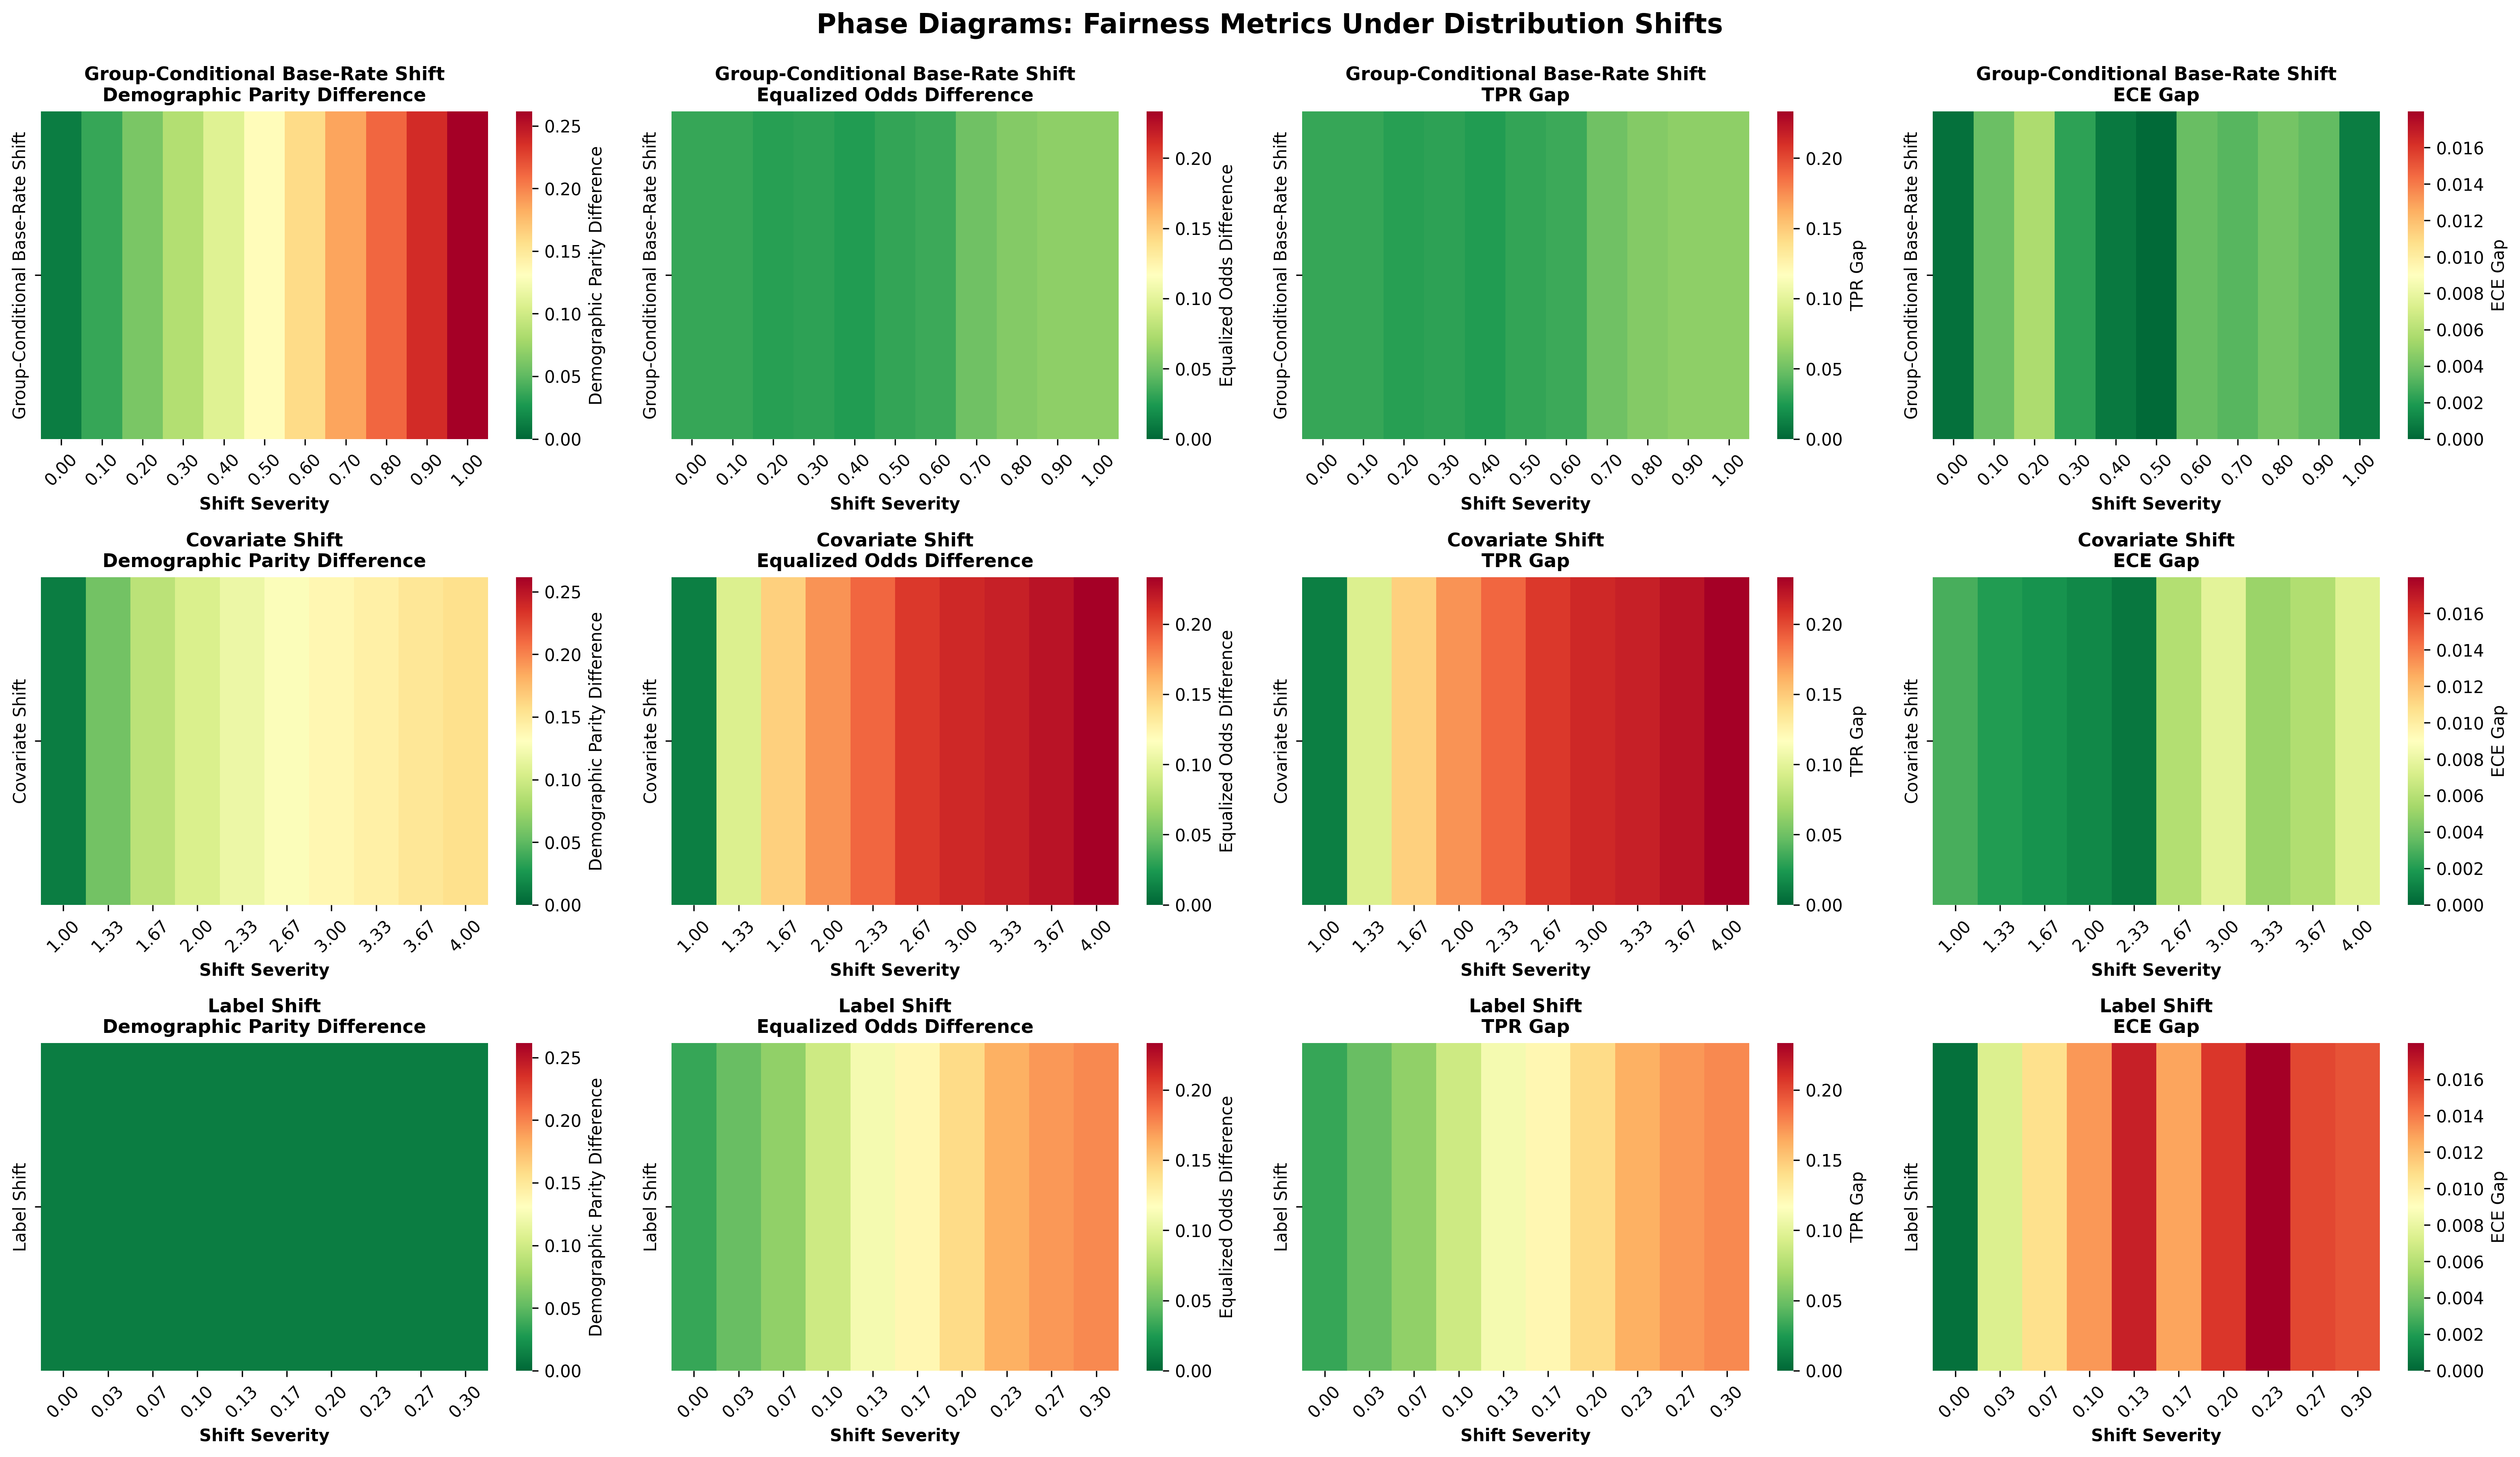
\includegraphics[width=1.0\textwidth]{figures/phase_diagrams.png}
    \caption{Metrics versus severity for the three one-dimensional extensions. Group-conditioned base-rate shift raises DP while the TPR gap changes modestly. Pure group-specific covariate shift raises DP and error-based gaps while the ECE gap remains small. Under asymmetric label noise, DP remains flat while the TPR gap computed from recorded labels rises sharply.}
    \label{fig:phase_diagram}
\end{figure}



\begin{figure}[h]
    \centering
    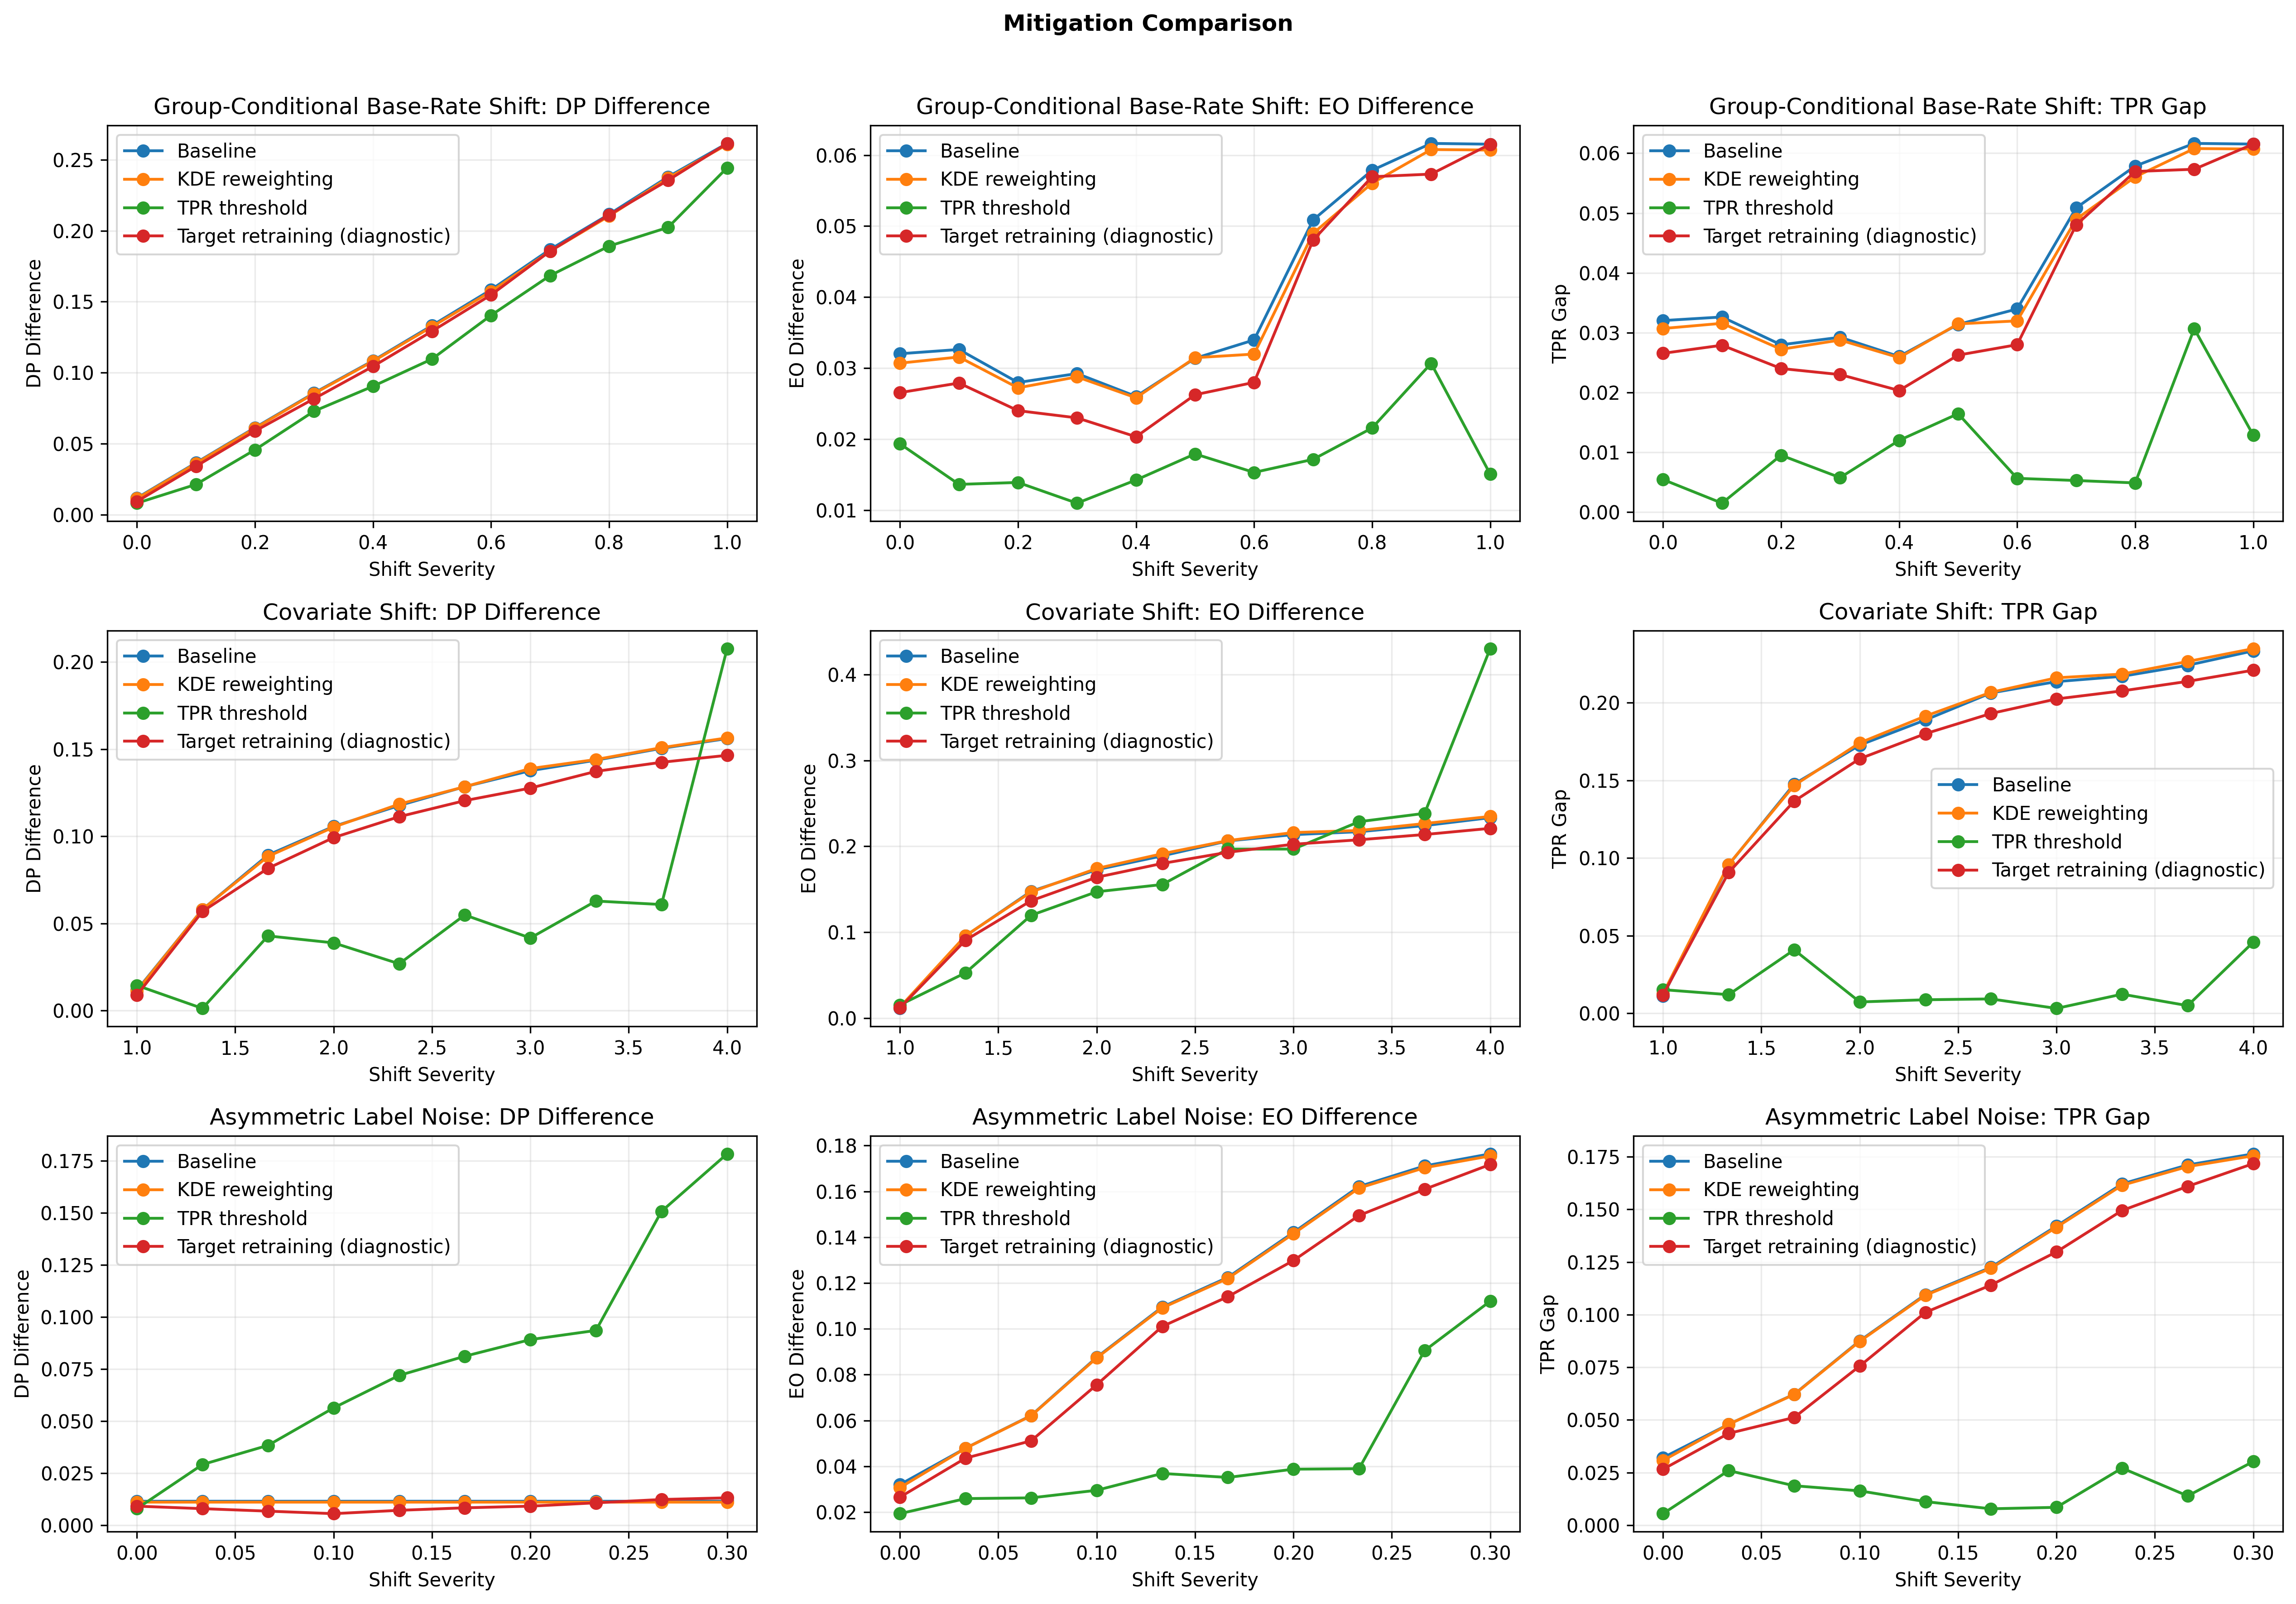
\includegraphics[width=1.0\textwidth]{figures/mitigation_comparison.png}
    \caption{Supplementary comparison across all shifts. KDE results outside pure covariate shift are negative controls rather than matched corrections. Threshold adjustment often reduces the TPR gap while increasing DP, FPR-driven EO, or both. Target retraining is a supervised reference, not a fairness-specific mitigation.}
    \label{fig:mitigation}
\end{figure}



\end{document}
